%\documentclass[landscape,a0b,final,a4resizeable]{a0poster}
\documentclass[landscape,a0b,final]{a0poster}
%\documentclass[portrait,a0b,final,a4resizeable]{a0poster}
%\documentclass[portrait,a0b,final]{a0poster}
%%% Option "a4resizeable" makes it possible ot resize the
%   poster by the command: psresize -pa4 poster.ps poster-a4.ps
%   For final printing, please remove option "a4resizeable" !!
\usepackage[danish]{babel} % dansk ordeling
\usepackage[utf8]{inputenc} % Read signs
\usepackage{amsmath}
\usepackage{amssymb}
\usepackage{bm}
\usepackage{multicol}
\usepackage{multirow}
\usepackage[usenames,dvipsnames]{color}
\usepackage{psfrag}
\usepackage{epsfig}
\usepackage{subfigure}
\usepackage{pstricks,pst-grad,calc}
\usepackage{algorithmic}
\usepackage{algorithm}
\usepackage{enumerate}
\usepackage{tikz}
\usetikzlibrary{arrows,shapes,snakes,automata,backgrounds,fit,petri}

% Definitions
\setlength{\columnsep}{3cm}
\setlength{\columnseprule}{2mm}
\setlength{\parindent}{0.0cm}

% Background
\newcommand{\background}[3]{
	\newrgbcolor{cbegin}{#1}
	\newrgbcolor{cend}{#2}
	\psframe[fillstyle=gradient, gradlines=1000, gradend=cend, gradbegin=cbegin,
           	 gradangle=0, gradmidpoint=#3]( 0., 0. )( 1.\textwidth, -1.\textheight )
}

% Poster environment
\newenvironment{poster}{
	\begin{center} \begin{minipage}[c]{0.98\textwidth} }{
	\end{minipage} \end{center}
}

% Custom column
\newenvironment{pcolumn}[1]{
	\begin{minipage}{#1\textwidth} \begin{center} }{
  	\end{center} \end{minipage}
}

% Custom box
\newcommand{\pbox}[4]{
	\psshadowbox[#3]{
		\begin{minipage}[t][#2][t]{#1}
			#4
		\end{minipage}
}}

% Custom section
\newcommand{\csection}[1]{
\vspace{1.25cm}
\begin{center}
	\pbox{0.8\columnwidth}{}{linewidth=2mm, framearc=0.0, linecolor=lightgreen, fillstyle=gradient,
	                         gradangle=0, gradbegin=white, gradend=whitegreen, gradmidpoint=1.0, framesep=0.6em, shadowsize=0
	                        }{\begin{center}{\bf #1}\end{center}}
\end{center}
\vspace{1.25cm}
}

% Custom caption
\setcounter{figure}{1}
\setcounter{table}{1}

\newcommand{\tcaption}[1]{
  \vspace{0.3cm}
  \begin{quote}
    {{\sc Table} \arabic{table}: #1}
  \end{quote}
  %\vspace{0.3cm}
  \stepcounter{table}
}

\newcommand{\fcaption}[1]{
  \vspace{0.3cm}
  \begin{quote}
    {{\sc Figure} \arabic{figure}: #1}
  \end{quote}
  \vspace{0.6cm}
  \stepcounter{figure}
}

\renewcommand\refname{ }

% Math definitions
%
% Useful definitions for vectors and stuff
%

% matrices and vectors
\def\A{{\bf A}}
\def\a{{\bf a}}
\def\B{{\bf B}}
\def\b{{\bf b}}
\def\C{{\bf C}}

\def\D{{\bf D}}
\def\E{{\bf E}}
\def\e{{\bf e}}

\def\F{{\bf F}}
\def\f{{\bf f}}
\def\G{{\bf G}}
\def\g{{\bf g}}
\def\H{{\bf H}}
\def\h{{\bf h}}
\def\I{{\bf I}}



\def\K{{\bf K}}
\def\k{{\bf k}}
\def\L{{\bf L}}

\def\M{{\bf M}}
\def\m{{\bf m}}




\def\P{{\bf P}}

\def\Q{{\bf Q}}
\def\q{{\bf q}}
\def\R{{\bf R}}
\def\r{{\bf r}}
\def\S{{\bf S}}
\def\s{{\bf s}}
\def\t{{\bf t}}
\def\U{{\bf U}}
\def\u{{\bf u}}
\def\V{{\bf V}}
\def\v{{\bf v}}
\def\W{{\bf W}}
\def\w{{\bf w}}
\def\X{{\bf X}}
\def\x{{\bf x}}
\def\Y{{\bf Y}}
\def\y{{\bf y}}
\def\Z{{\bf Z}}
\def\z{{\bf z}}

% permutations
\def\PL{{\bf P}_\mathrm{r}}
\def\PR{{\bf P}_\mathrm{c}}
\def\PC{{\bf P}_\mathrm{f}}

% more stuff
\def\BNet{{\cal B}}
\def\GR{{\cal D}}
\def\ED{{\cal E}}
% \def\S{{\cal S}}
\def\VR{{\cal V}}
\def\Sp{{\cal S}}
\def\0{{\bf 0}}
\def\1{{\bf 1}}

\def\Re{\mathbb{R}}
\def\Ex{\mathbb{E}}
\def\Lik{\mathcal{L}}

\def\<{\, \langle \,}
\def\>{\, \rangle \,}
\def\inv{^{-1}}
\def\ts{^\top}
\def\lik{{\cal L}}
\def\topc{\mathrm{top}}

% mathrms
\def\sign{\mathrm{sign}}
\def\max{\mathrm{max}}
\def\min{\mathrm{min}}
\def\tr{\mathrm{trace}}
\def\diag{\mathrm{diag}}
\def\MAP{\mathrm{MAP}}
\def\ICA{\mathrm{ICA}}
\def\FM{\mathrm{FM}}
\def\DAG{\mathrm{DAG}}
\def\FA{\mathrm{FA}}
\def\BN{\mathrm{BN}}
\def\rep{\mathrm{rep}}
\def\block{\mathrm{block}}
\def\abs{\mathrm{abs}}

% bold greeks
\def\balpha{\bm{\alpha}}
\def\bbeta{\bm{\beta}}
\def\bPsi{\bm{\Psi}}
\def\bSigma{\bm{\Sigma}}
\def\bepsilon{\bm{\epsilon}}
\def\bupsilon{\bm{\upsilon}}
\def\bmeta{\bm{\eta}}
\def\bmu{\bm{\mu}}
\def\bnu{\bm{\nu}}
\def\btau{\bm{\tau}}
\def\bLambda{\bm{\Lambda}}
\def\bTheta{\bm{\Theta}}

% distributions
\def\DN{\mathcal{N}}
\def\TN{\mathcal{TN}}
\def\IG{\mathrm{IG}}
\def\La{\mathrm{Laplace}}
\def\Exp{\mathrm{Exponential}}
\def\Uni{\mathrm{Uniform}}
\def\Be{\mathrm{Beta}}
\def\Bin{\mathrm{Binomial}}
\def\Ber{\mathrm{Bernoulli}}
\def\Ga{\mathrm{Gamma}}
\def\Poi{\mathrm{Poisson}}
\def\GP{\mathrm{GP}}
\def\DP{\mathrm{DP}}
\def\TP{\mathrm{TP}}
\def\IGamma{{\cal IG}}
\def\DGamma{{\cal G}}
\def\Wish{\mathrm{Wishart}}
\def\IW{{\cal IW}}
\def\MOD{\mathcal{M}}
\def\LN{\mathrm{logNormal}}

% commands
\newcommand{\argmax}{\operatornamewithlimits{argmax}}
\newcommand{\argmin}{\operatornamewithlimits{argmin}}
\newcommand{\deff}{\overset{\underset{\mathrm{def}}{}}{=}}
\newcommand{\indi}{\overset{\underset{\mathrm{ind}}{}}{\sim}}
\newcommand{\Perp}{\perp \! \! \! \perp}

\newcommand{\ie}{i.e. }
\newcommand{\eg}{e.g. }
\newcommand{\wrt}{w.r.t. }
\newcommand{\iid}{i.i.d. }

\newcommand{\tmp}[1]{{\color{orange} {\bf #1}}}
\newcommand{\quotes}[1]{``#1''}

\def\ctilde{\kern -.04em\lower .7ex\hbox{\~{}}\kern .04em}

\def\Tiny{\fontsize{5pt}{5pt}\selectfont}


\begin{document}

\background{0.988 0.988 0.988}{0.933 0.933 0.933}{1.0}
\vspace*{1cm}

\newrgbcolor{lightblue}{0. 0. 0.80}
\newrgbcolor{white}{0.988 1.000 0.960}
\newrgbcolor{whiteblue}{.80 .80 1.}
\newrgbcolor{lightgreen}{0.349 0.376 0.431}
\newrgbcolor{whitegreen}{0.678 0.658 0.580}

\begin{poster}
%
\begin{center}
\begin{pcolumn}{0.99}
%
\pbox{0.95\textwidth}{}{linewidth=2mm, framearc=0.0, linecolor=lightgreen, fillstyle=gradient,
                        gradangle=0,gradbegin=white,gradend=whitegreen,gradmidpoint=1.0,framesep=0.5em,shadowsize=0}
{
% University logo
\begin{minipage}[c][7cm][c]{0.1\textwidth}
	\begin{center}
    	
\includegraphics[width=12cm,angle=0]{images/dtu_logo}
	\end{center}
\end{minipage}
% Title and Authors
\begin{minipage}[c][7cm][c]{0.78\textwidth}
 	\begin{center}
    	{\huge {\bf Leverage based sampling for classification} } \\ [6.5mm]
    	{\Large  Julian Kopka Larsen and Jesper Løve Hinrich . \\ \emph{Superviser} Lars Kai Hansen} \\ [5.5mm]
     	\begin{tabular}{cc}
			DTU Compute $\cdot$ Technical University of Denmark \\
			Kgs. Lyngby, Denmark & Copenhagen N, Denmark
		\end{tabular}
  	\end{center}
\end{minipage}
% Department logo
\begin{minipage}[c][7cm][c]{0.1\textwidth}
	\begin{center}
   		
\includegraphics[width=12cm,angle=0]{images/dtucompute_logo}
	\end{center}
\end{minipage}
%
}
\end{pcolumn}
\end{center}
%
\vspace*{0.5cm}
%
\begin{multicols}{3}
%
\csection{Abstract}
%
We validate the results of leverage based sampling for LS-regression, shown by Ma et al. [1]. We explore the possibility of using the leverage based sampling distribution from LS-regression on 2 class classification, and introduce a new approach for sampling from an leverage distribution (important points).
%
\csection{Motivation}
The importance of sampling methods is initiated by very large datasets where it is not feasible to use all of the available data. This is illustrated by the rise in online access to video data. These data contain many frames that are basically the same and therefore redundant. 
%
\csection{Concept}
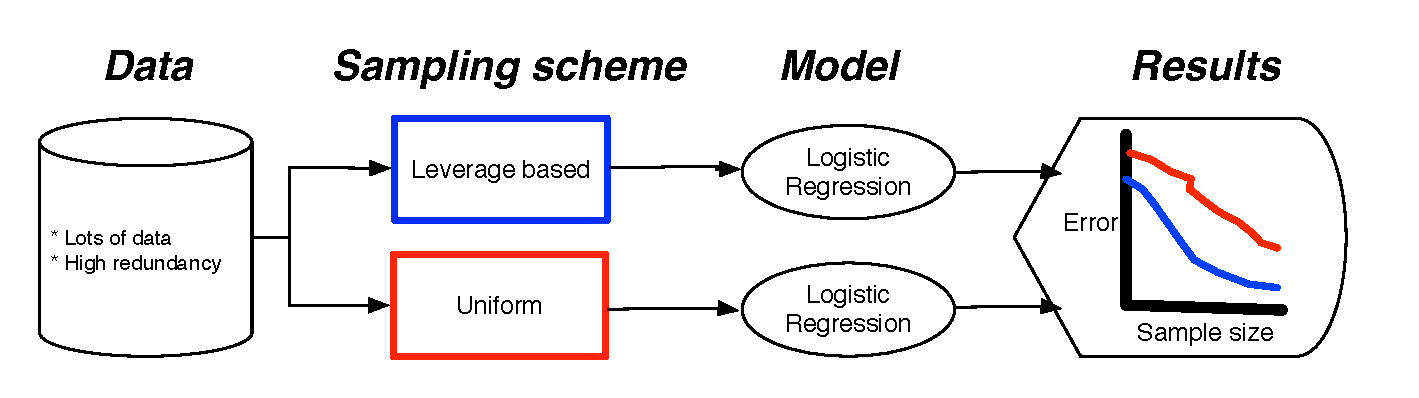
\includegraphics[width=.95\linewidth]{images/ThoughtModel}
%
\csection{Research Questions}
\begin{itemize}
	\item Will the regression based sampling distribution improve our performance in classification?
	\item Can leverage based sampling be generalized to classification?
\end{itemize}
%
\csection{Datasets}
%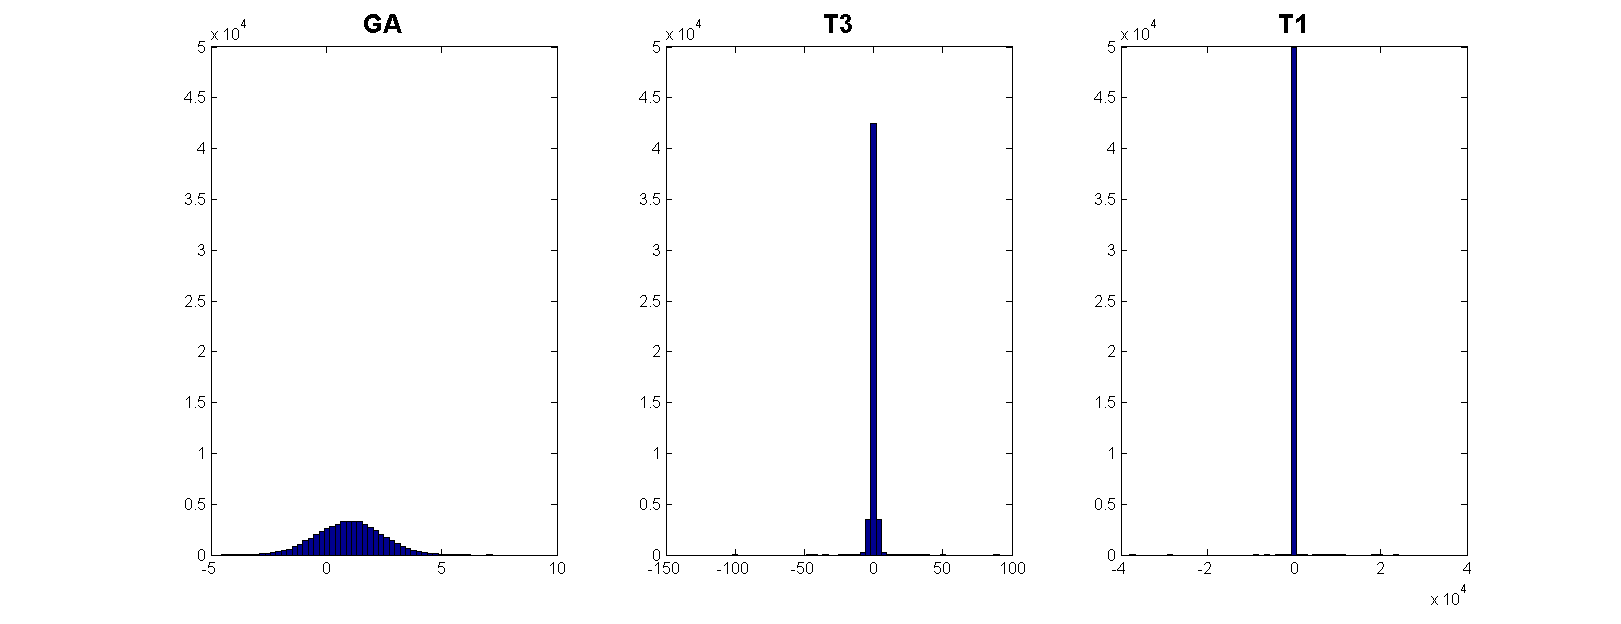
\includegraphics[width=\linewidth]{images/Data_distributions.png}
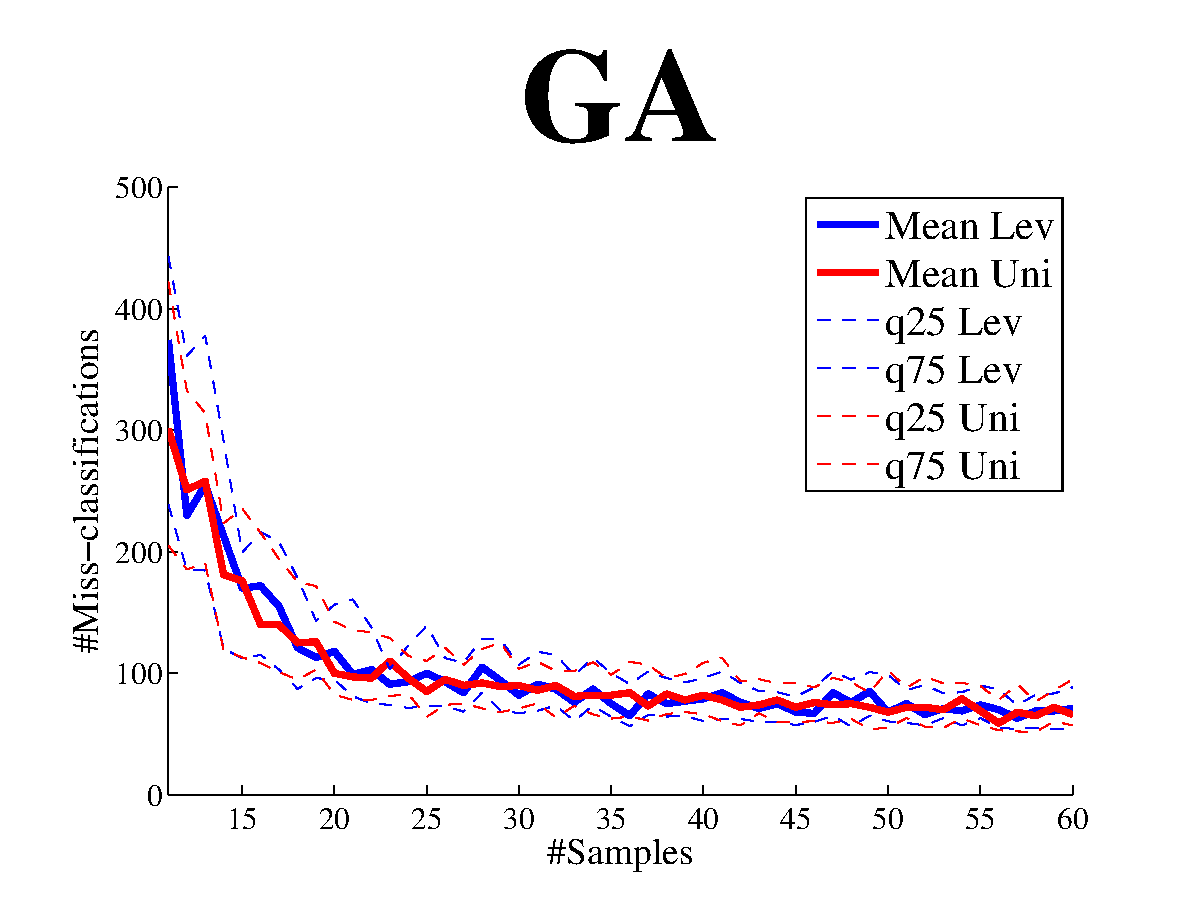
\includegraphics[width=0.32\linewidth]{images/GA.eps}

These datasets are drawn from distributions defined in Ma et al. \cite{Ma} and have:

\begin{itemize}
	\item GA: Nearly uniform leverage-scores
	\item T3: Mildly non-uniform leverage-scores
	\item T1: Very non-uniform leverage-scores
\end{itemize}  
%
\csection{Leveraging in for least squares regression}
For any leveraging we want to find for each datapoint a leverage-score representing the importance of the point. This we can normalize into a distribution to sample from.
%
\csection{Validating the results of Ma et al.}
\begin{figure}[H]
\centering
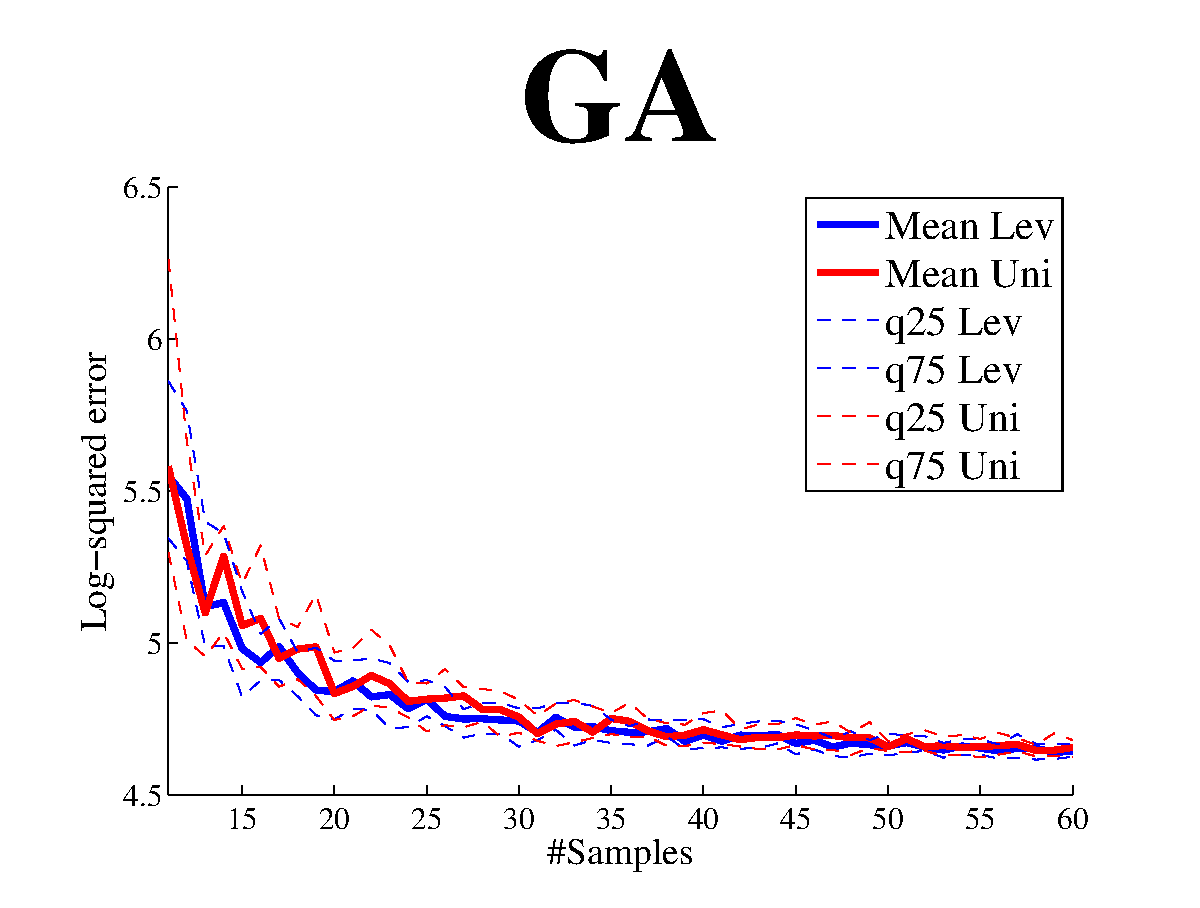
\includegraphics[width=.32\linewidth]{images/GALS.eps}
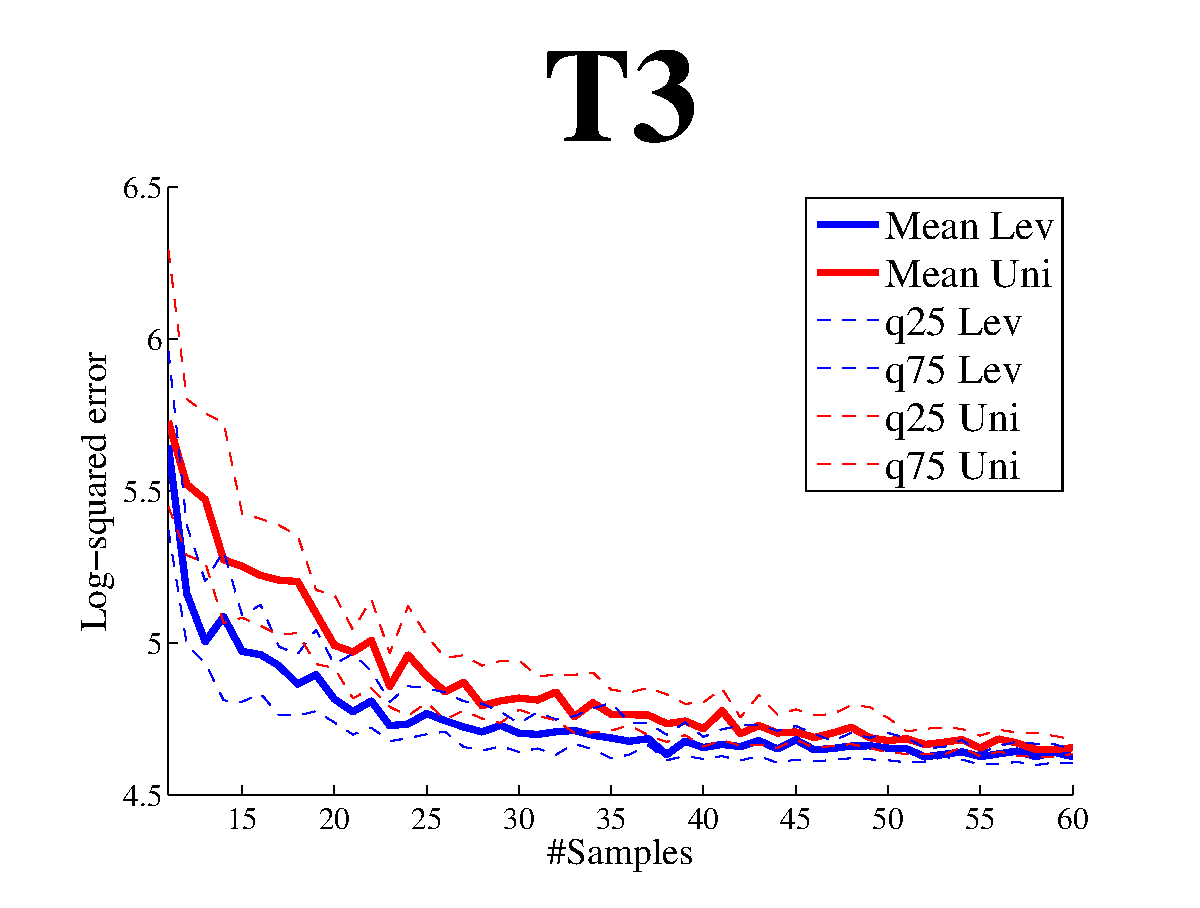
\includegraphics[width=.32\linewidth]{images/T3LS.eps}
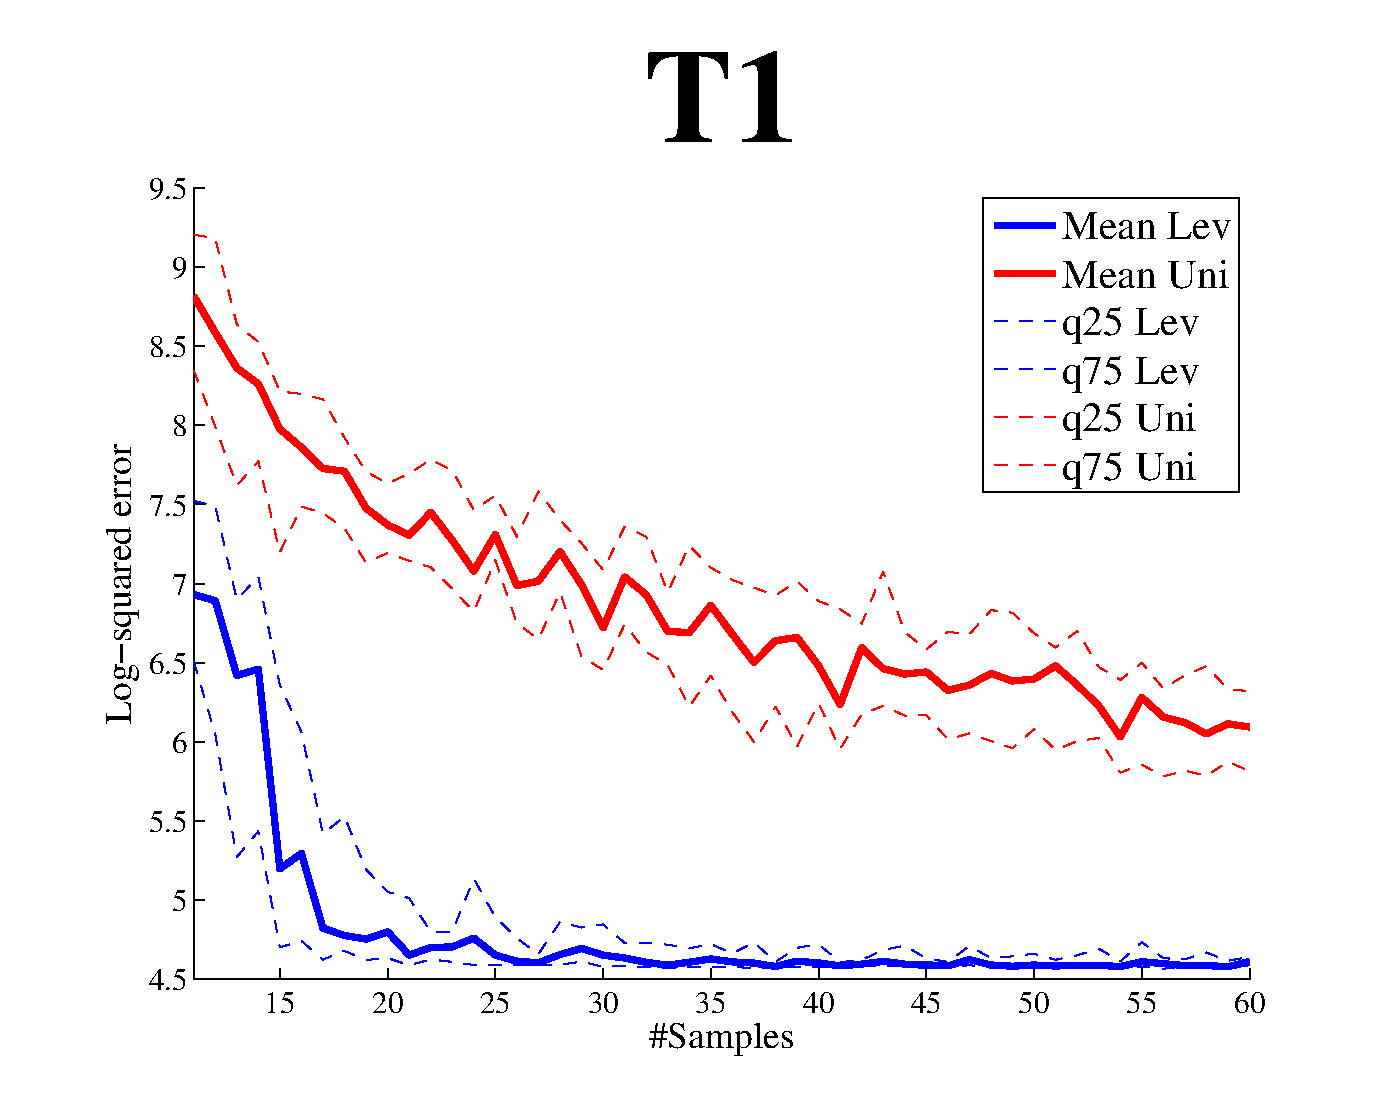
\includegraphics[width=.32\linewidth]{images/T1LS.eps}
\caption{Lal di la}
\end{figure}

%
\csection{LS-based Distribution}
We seek to find the effect that a datapoint's class has on the predicted class for that datapoint.
	    \begin{equation}
	    \label{dyhatdy}
	    \frac{\delta \hat{y}_n}{\delta y_n}
	    \end{equation}
	There is a closed form solution which is linear in $y$
		\begin{equation*}
			\hat{\beta}_{OLS} = \left( X^T X \right)^{-1} X^T y \quad \text{where} \quad \hat{y}_n = X_n*\hat{\beta}
		\end{equation*}
		
	Therefore the leverage-score \eqref{dyhatdy} is the coefficient
		\begin{equation*}
			\frac{\delta \hat{y}_n}{\delta y_n} = X \left( X^T X \right)^{-1} X^T
		\end{equation*}
%
\csection{Test Results}
We compared logistic regression when sampling from a LS-distribution (blue) vs. a uniform-distribution (red). The mean, 25th and 75th quantile are plotted.\\
	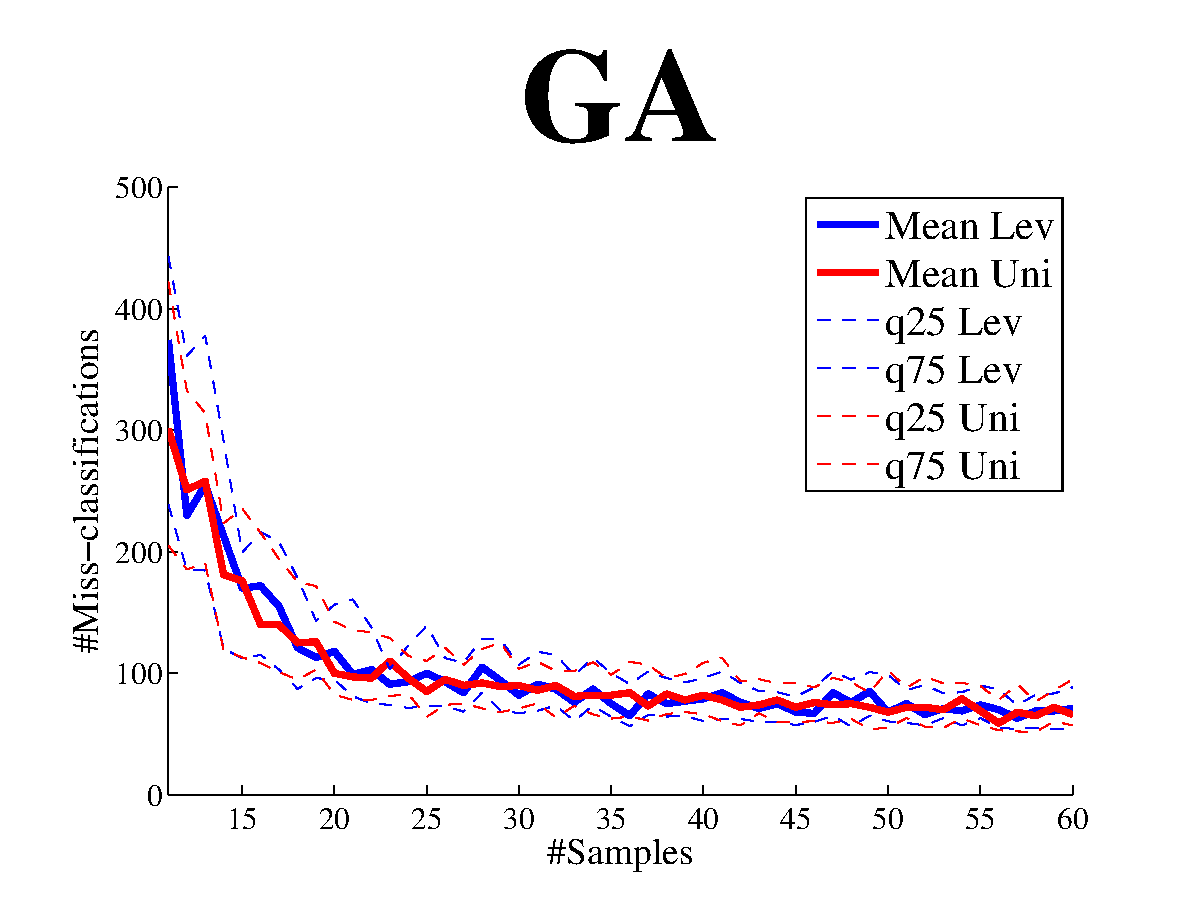
\includegraphics[width=.32\linewidth]{images/GA.eps}	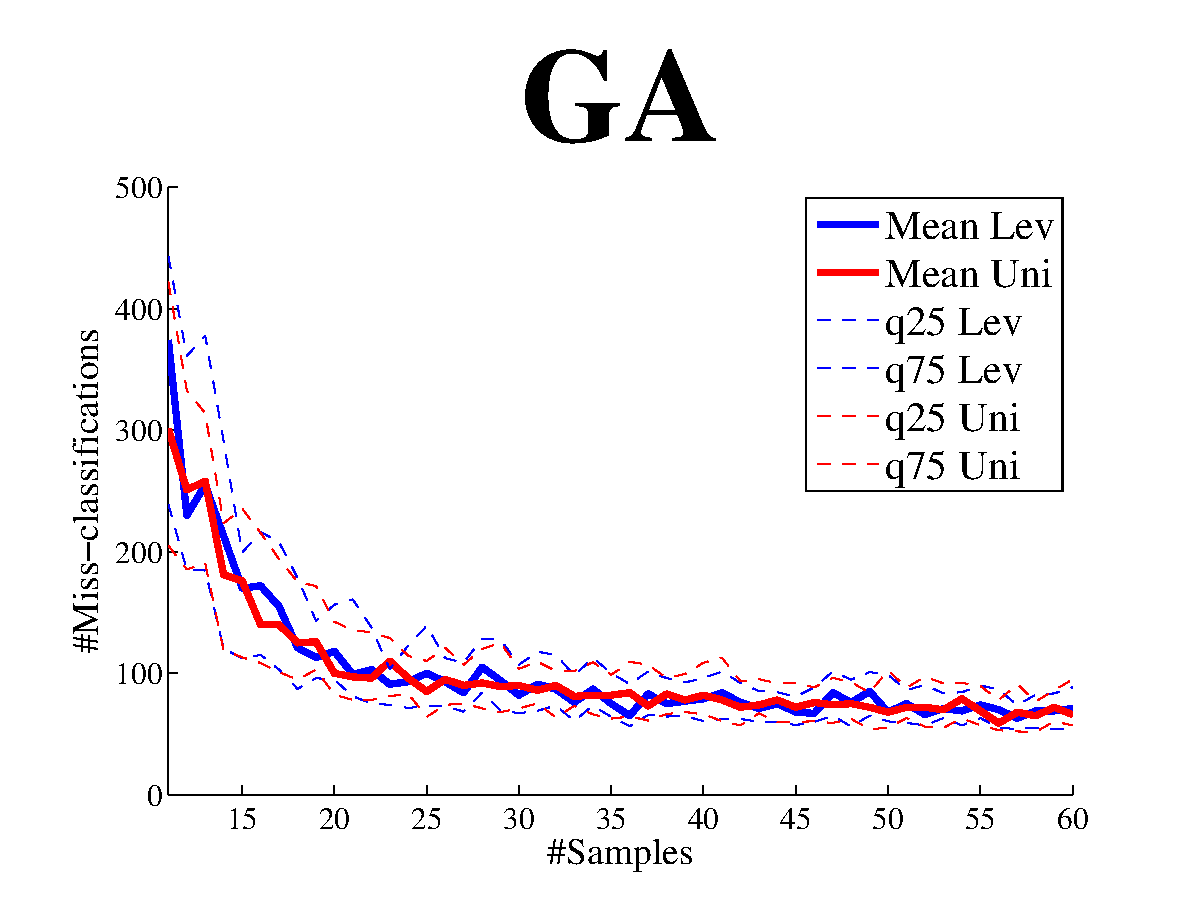
\includegraphics[width=.32\linewidth]{images/GA.eps}	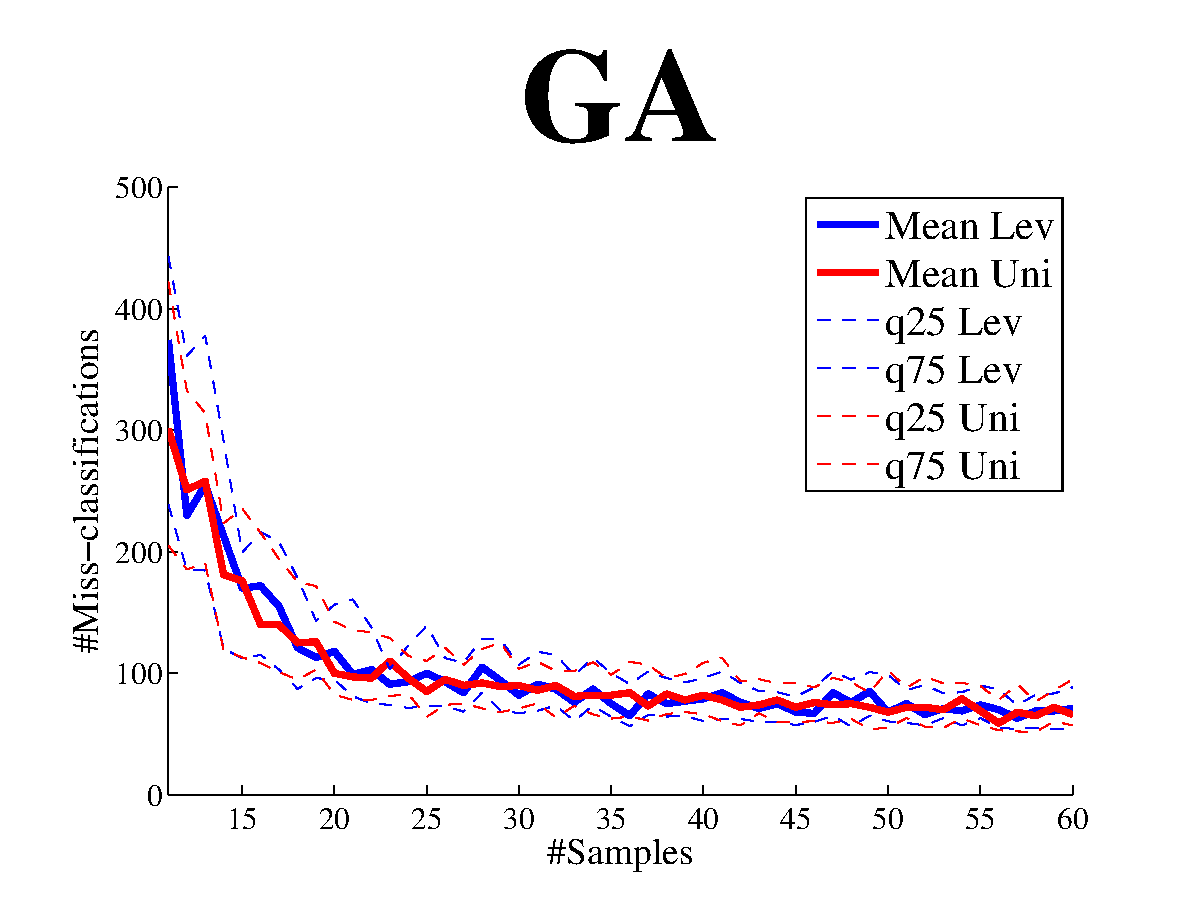
\includegraphics[width=.32\linewidth]{images/GA.eps}\\
	It clearly shows that a LS-distribution sample scheme, does not outperform a uniform-distribution for classification. The results shown are for dimension $p = 10$ and $N = 1000$ datapoints, but it is consistent when varying $p$ and $N$. 
%
\csection{Sensitivity Based Distribution}
Vi generalisere til noget andet, og derfor kan WLS ikke bruges, så vi laver bare LS.
The target is again \eqref{dyhatdy} 
    	\begin{equation*}
    	\label{optimum}
    	 \hat{y}_n = p(y|\bar{x},\bar{w}) \quad \bar{w} \  \text{s.t.} \ \frac{\delta L}{\delta\bar{w}}=0
    	\end{equation*}
    	Since \ref{optimum} depends both directly and indirectly on $y$ we see that
    	\begin{eqnarray*}
    	&\frac{\delta}{\delta y} \frac{\delta L}{\delta w} = 0\\
    	\Downarrow & \\
    	&\frac{\delta^2 L}{\delta y \delta \bar{w}} + \frac{\delta^2 L}{\delta \bar{w} \delta \bar{w}^T} \frac{\delta \bar{w}}{\delta y}= 0
    	\end{eqnarray*}
    	
    	and from this we can get our leverage-score \eqref{dyhatdy}
    	
    	\begin{equation*}
    		\frac{\delta \hat{y}_n}{\delta y_n}=\frac{\delta p(y|\bar{x}_n,\bar{w})}{\delta \bar{w}^T} \frac{\delta \bar{w}}{\delta y} = - \frac{\delta p(y|\bar{x}_n,\bar{w})}{\delta \bar{w}^T} \left[ \frac{\delta^2 L}{\delta \bar{w} \delta \bar{w}^T} \right]^{-1} \frac{\delta^2 L}{\delta y \delta \bar{w}}
    	\end{equation*}
    	
    	When evaluating this model, weights trained on a small training-set is used. This is expected to be better than LS-based sampling since it introduces dependence on class information.
%
\csection{Conclusion}
The LS-based leverage sampling gives no advantage over uniform sampling and generally performs worse. LS-distribution is based on what is important for linear regression, it does not have an advantage in finding important points for classification.

\csection{References}
%
\vspace{-2.5cm}
\bibliographystyle{is-unsrt}
%\footnotesize{
\bibliography{./mlbib}
%}
%
\end{multicols}
%
\end{poster}
%
\end{document}
